\section{Key/value cache servers}
\label{sec:server}

To demonstrate the benefits of \cphash{} in an application we developed
\cpserver{}, a \memcached{}-style Key/Value Cache Server, which uses \cphash{} to
implement its hash table.  For comparison, we also implemented a version of this
server in a shared-memory style using fine-grained locking.
Section~\ref{sec:eval} compares these two implementations with \memcached{}.

\subsection{{\cpserver}{}}

Figure \ref{fig:mcserver} shows the design of \cpserver{}.  \cpserver{} has
server and client threads as described in Section~\ref{sec:design}. TCP clients
on client machines connect to the server using TCP connections.  A client thread
monitors TCP connections assigned to it and gathers as many requests as possible
to perform them in a single batch. Then, a client thread passes the back of
requests to the appropriate server threads using message passing. After a server
thread is done and the client thread receives their results back, the client
threads writes back those results to the appropriate TCP connections.

The \cpserver{} also has a TCP server thread that accepts new connections. When
a connection is made, it is assigned to a client thread with the smallest number
of current active connections.  The load balancer could be more advanced for
work loads in which the traffic on different connections differ significantly.

\begin{figure}[!ht]
  \centering
  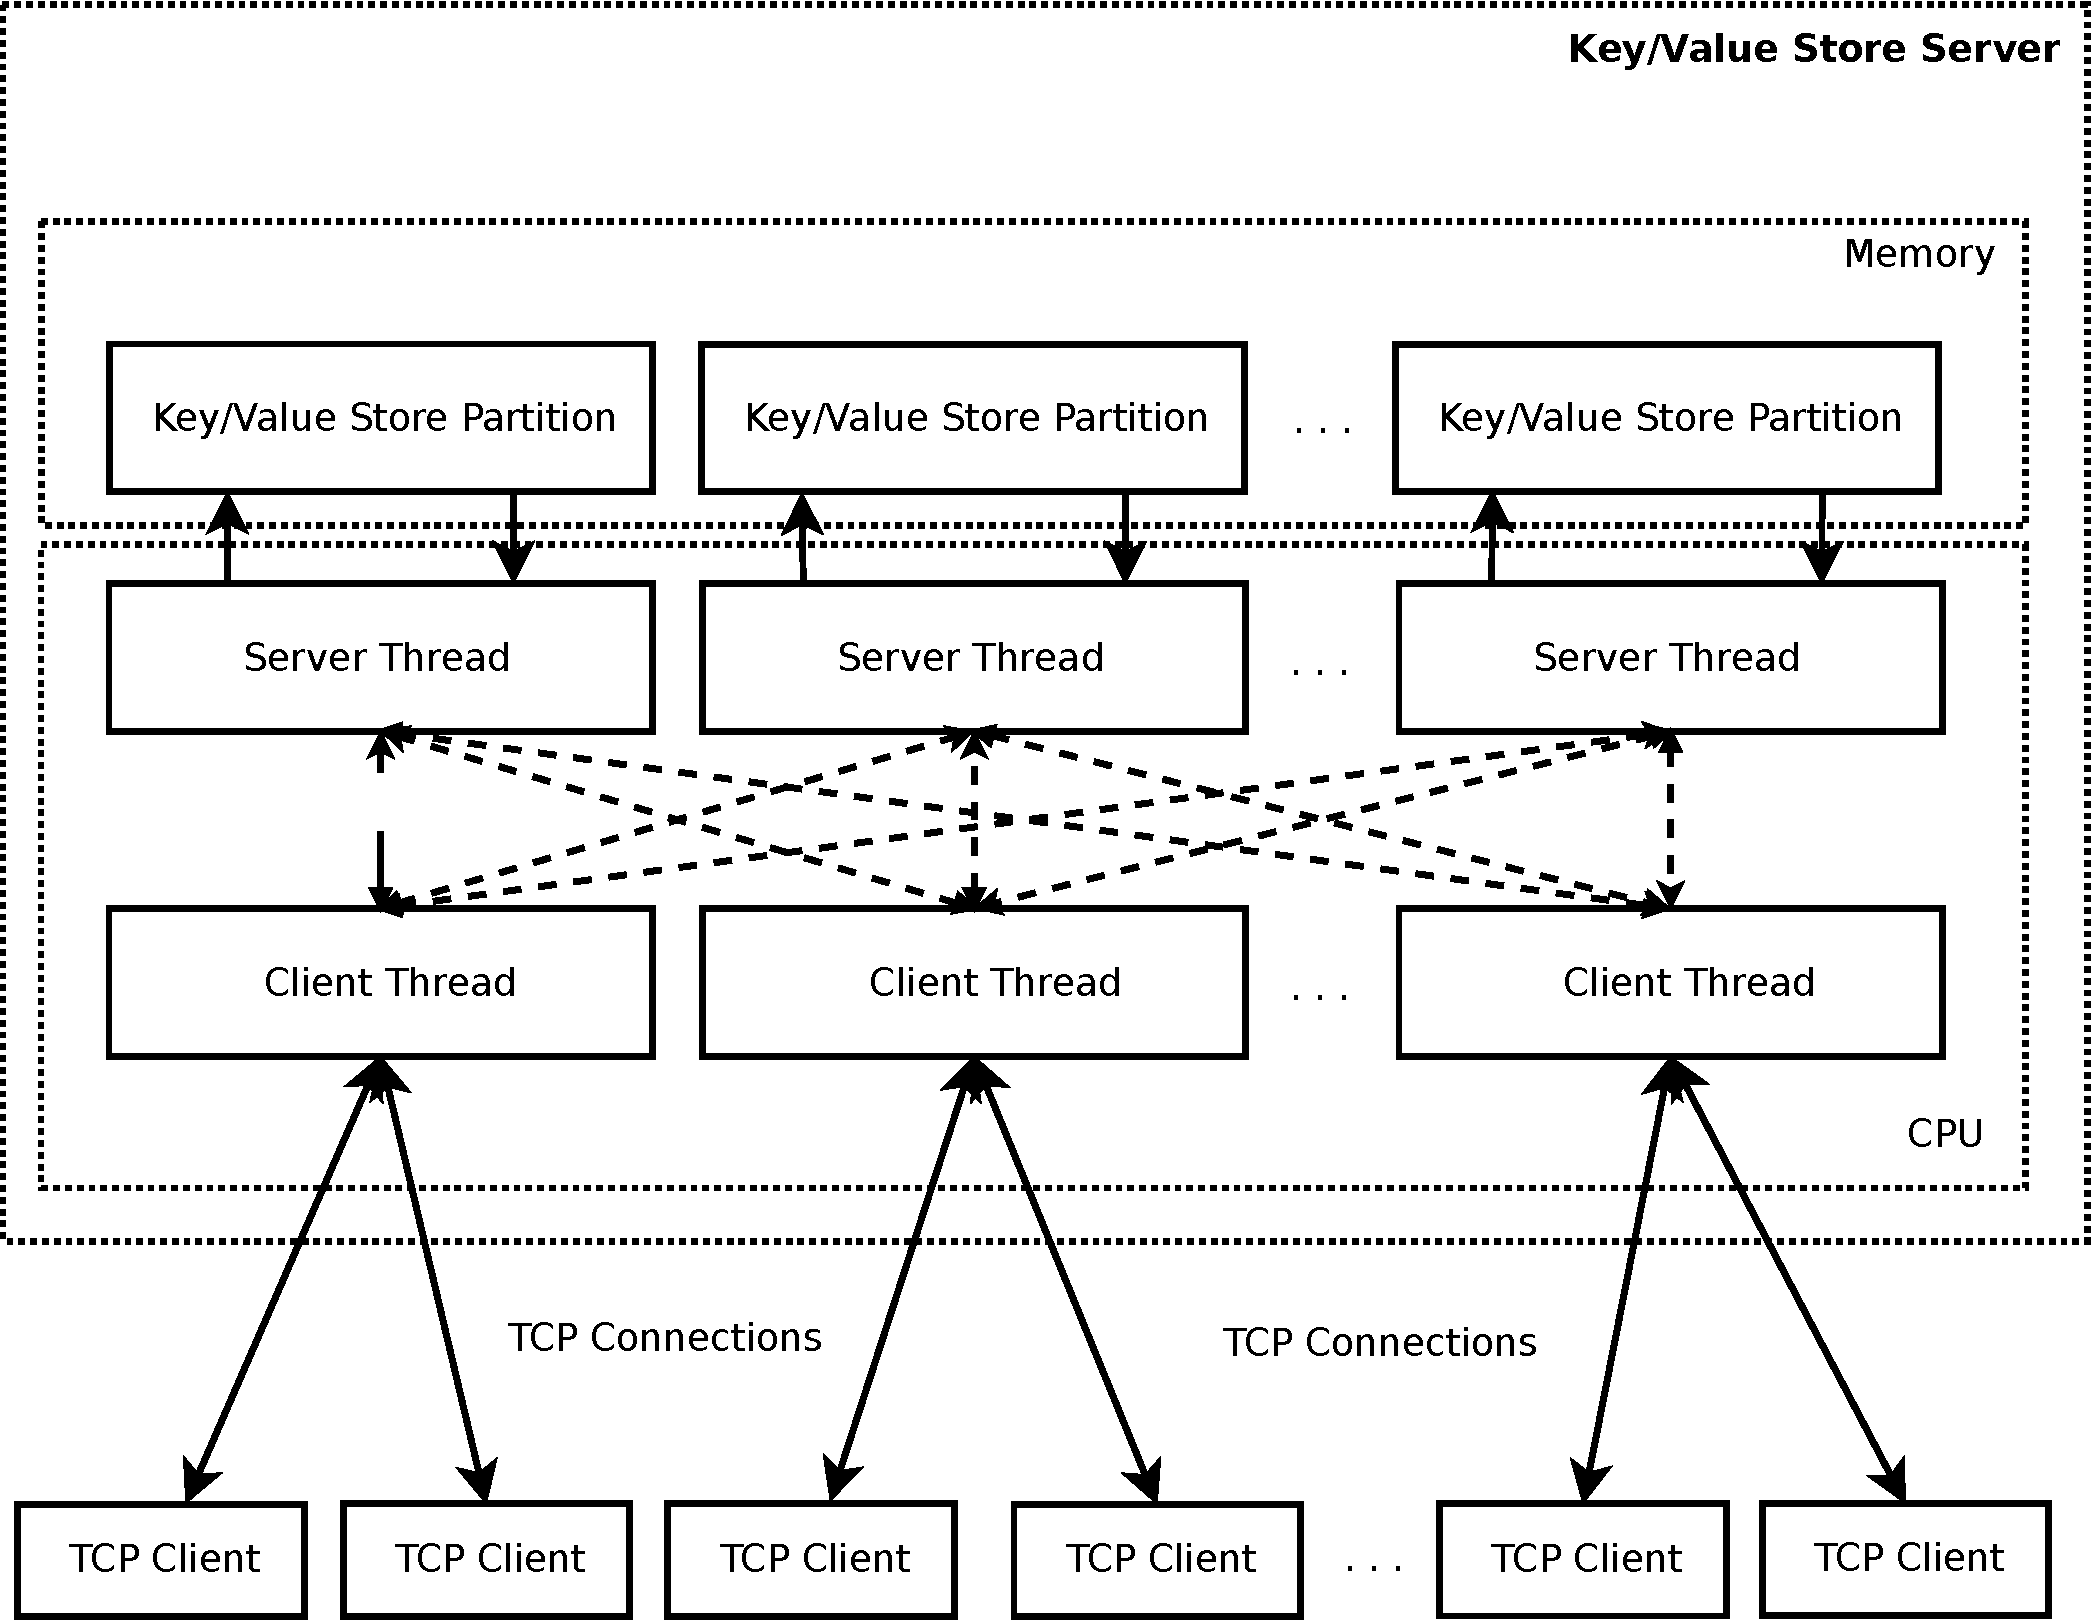
\includegraphics[width=\linewidth]{figs/mcserver.pdf}
  \caption{\cpserver{} design}
  \label{fig:mcserver}
\end{figure}

\cpserver{} uses a simple binary protocol with two message types:
\begin{description}

\item[LOOKUP] With the LOOKUP request the TCP client asks the server to try to
  find a key/value pair in the hash table such that the key matches the
  \texttt{hash key} field from the request. The \texttt{size} field is unused
  for the LOOKUP request, thus it can be set to any value.  If the requested
  key/value pair is found in the hash table, then the server returns the size of
  the value and the actual value data are returned.  Otherwise, the server
  returns a response with a \texttt{size} of 0 is returned.

\item[INSERT] With the INSERT request the TCP client asks the server to insert a
  new key/value pair in the hash table.  The \texttt{hash key} field is the key
  to be inserted. The \texttt{size} field is the size of the value to be
  inserted in the hash table.  The INSERT request header is followed by
  \texttt{size} amount of bytes which describe the value to be inserted. The
  INSERT requests are silent, and the server returns no response.
  the server.

\end{description}

\subsection{\lockserver{}}

To evaluate the performance and scalability of \cphash{}, we created
\lockserver{}, which does not use message passing. It supports the same
protocol, but uses a shared-memory style hash table, which we name
\lockhash{}, with scalable fine-grained locks.  To make the comparison fair,
\lockhash{} also has $n$ LRU lists instead of 1 global one, by dividing the hash
table into $n$ partitions.  Each partition is protected by a lock to protect the
LRU list for that partition.The client threads of \lockserver{} process queries
by first acquiring the lock for the appropriate partition, then performing the
query, updating the LRU list and, finally, releasing the lock.  \XXX{maybe no
  contention if we random replacement and a lock per bucket.  as is \lockhash{}
  isn't particular fine-grained}

